\section{Transformer}
\label{sec:transformer}
“Attention is All you Need” (Vaswani, et al., 2017) \cite{vaswani2017attention}, is impactful work in both natural language processing or computer vision field. It presented a lot of improvements and the proposed “transformer” model is entirely built on the self-attention mechanisms without using sequence-aligned recurrent architecture (which will describe in section \ref{subsec:attention}). The Transformer model has an encoder-decoder architecture, as commonly used in many natural machine translation models. Later decoder-only Transformer was shown to achieve great performance in language modeling tasks, like in GPT and BERT. Nowadays, transformer also use in computer vision because of the context-understanding ability of it and become one of the state-of-the-art.

\subsection{Sequence to sequence (Seq2Seq)}
The seq2seq model was introduced by Sutskever \cite{sutskever2014sequence}, et al in the language modeling field. It tackle the transformation of an source sequence to a target one, firsly apply in neural machine translation (figure \ref{fig:seq2seq}). The seq2seq model normally has an encoder-decoder architecture, composed of:

\begin{itemize}
    \item \textbf{Encoder}: to compress the information of input sequence and represent it as an context vector. This representation is expected to be summery the whole source sequence.
    \item \textbf{Decoder}: is initialized with the context vector to emit the transformed output. Seq2seq only used the last embedding state of the encoder network as the decoder initial input.
\end{itemize}
\begin{figure}
    \centering
    \includegraphics{}
    \caption{The sequence to sequence overview}
    \label{fig:seq2seq}
\end{figure}
This architecture is the foundation of many sequential models nowadays, but still exist few limitations such as use a fixed-length context vector. And one of the the most improvements handle this problem is attention mechanism.

\subsection{Attention and Self-Attention mechanism}
\label{subsec:attention}
\textbf{The attention mechanism} uses to memorize long source sentences in neural machine translation. Define the attention mechanism in a scientific way. Say, we have source sequence \mathbf{x} have length $n$ and target sequence \mathbf{y} have length $m$
\begin{equation}
\mathbf{x} &= [x_1, x_2, \dots, x_n] \text{;}
\mathbf{y} &= [y_1, y_2, \dots, y_m]
\end{equation}

The key idea is it create weighted shortcuts between the context vector and the entire source input. The alignment between the source and target is learned by a context vector. The context vector is a sum of hidden states $\boldsymbol{h}_i$ of the encoder sequence and weighted by alignment scores $\alpha_{t,i}$, in there $\alpha_{t_i}$ is calculate from the hidden states $\boldsymbol{s}_i$ from the decoder. 

\begin{equation}
\label{eq:align_score}
\mathbf{c}_t &= \sum_{i=1}^n \alpha_{t,i} \boldsymbol{h}_i & \small{\text{; Where $c_t$ is the context vector for output }y_t}
\end{equation}

The alignment score $\alpha_{t,i}$ is assign by a model to the pair of input at position and output at position based on how well they match. The set of pairs are weights how much of each source hidden state should be considered for each output. The score function is therefore in the following form below at timestamp $t$:
\begin{equation}
    e_{ij}=a(s_i,h_j), \qquad \alpha_{i,j}=\frac{\exp(e_{ij})}{\sum_k\exp(e_{ik})}
\end{equation}

\textbf{Self-attention} is an attention mechanism variant, in that it relating different positions of a single sequence in order to compute a representation of the same sequence. The self-attention mechanism use to learn the correlation between the current token and the previous part of the sequence. 

\subsection{Multi-head Self-Attention}
In the paper attention is all you need, transformer component have re-define the attention by using retrieval concept. The encoded representation of the input as a set of key-value pairs $\mathbf{K}, \mathbf{V}$.
In the decoder, the previous output is compressed into a query $\mathbf{Q}$ and the next output is produced by mapping this query and the set of keys and values.  

\begin{equation}
    \text{Attention}(\mathbf{Q}, \mathbf{K}, \mathbf{V}) = \text{softmax}(\frac{\mathbf{Q}\mathbf{K}^\top}{\sqrt{n}})\mathbf{V}
\end{equation}
Where $n$ is the dimension of the source hidden state. And we have a scalar score $a_{ij}$ follow
\begin{equation}
    a_{ij} = \text{softmax}(\frac{\mathbf{q}_i {\mathbf{k}_j}^\top}{\sqrt{n}})
= \frac{\exp(\mathbf{q}_i {\mathbf{k}_j}^\top)}{ \sqrt{n} \sum_{r \in S_i} \exp(\mathbf{q}_i {\mathbf{k}_r}^\top) }
\end{equation}
The reason behind this because the attention operation can be thought of as a retrieval process as well. As mention in eq \ref{eq:align_score}, if we remove the constraint that the weight $\alpha_{t}$ is a one-hot vector, the operation could be thought as a retrieval process according to the $\alpha_{t}$ as a probability vector. This way efficiency computes the vector $\alpha_{t}$ as a matrix multiply to measure the similarity by project $s$ and $h$ to a common space instead of we have to go through the network $n \times m$ times to acquire all the attention scores $a_{ij}$.
\begin{equation}
    \label{eq:scale_dot_product}
    \text{score}(\boldsymbol{s}_t, \boldsymbol{h}_i) = \frac{\boldsymbol{s}_t^\top\boldsymbol{h}_i}{\sqrt{n}}
    \caption{Scaled dot-product formula}
\end{equation}
\textbf{The multi-head self-attention module} is a key component in transformer. In summary, the idea of multi-head attention is to split the feature dimension of the input into many parts and attention over these sub-dimensions. Then computes the scaled dot-product attention (eq \ref{eq:scale_dot_product}) over each subspace in parallel. Each independent attention outputs are simply concatenated and linearly transformed into expected dimensions.
\begin{figure}[h]
    \centering
    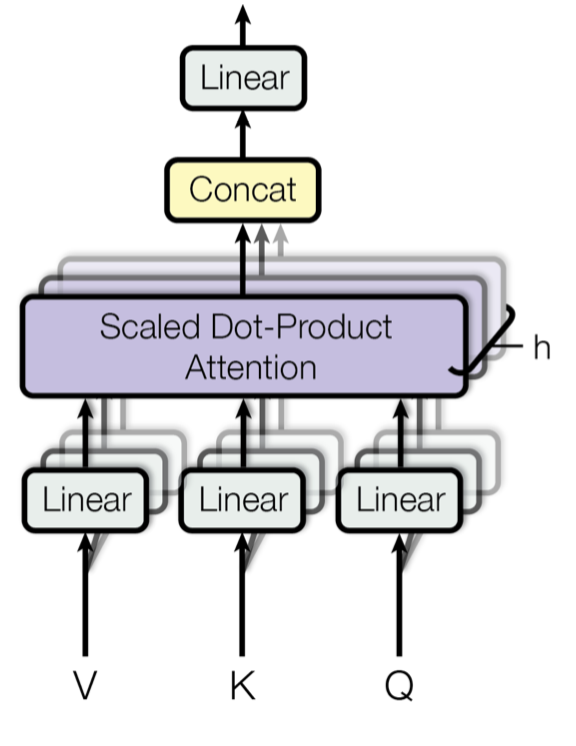
\includegraphics[height=2in]{content/resources/new_images/background/multi-head-attention.png}
    \caption{Multi-head scaled dot-product attention mechanism \cite{vaswani2017attention}}
    \label{fig:multiheadatt}
\end{figure}
\subsection{Transformer architecture}

\begin{figure}[h]
    \centering
    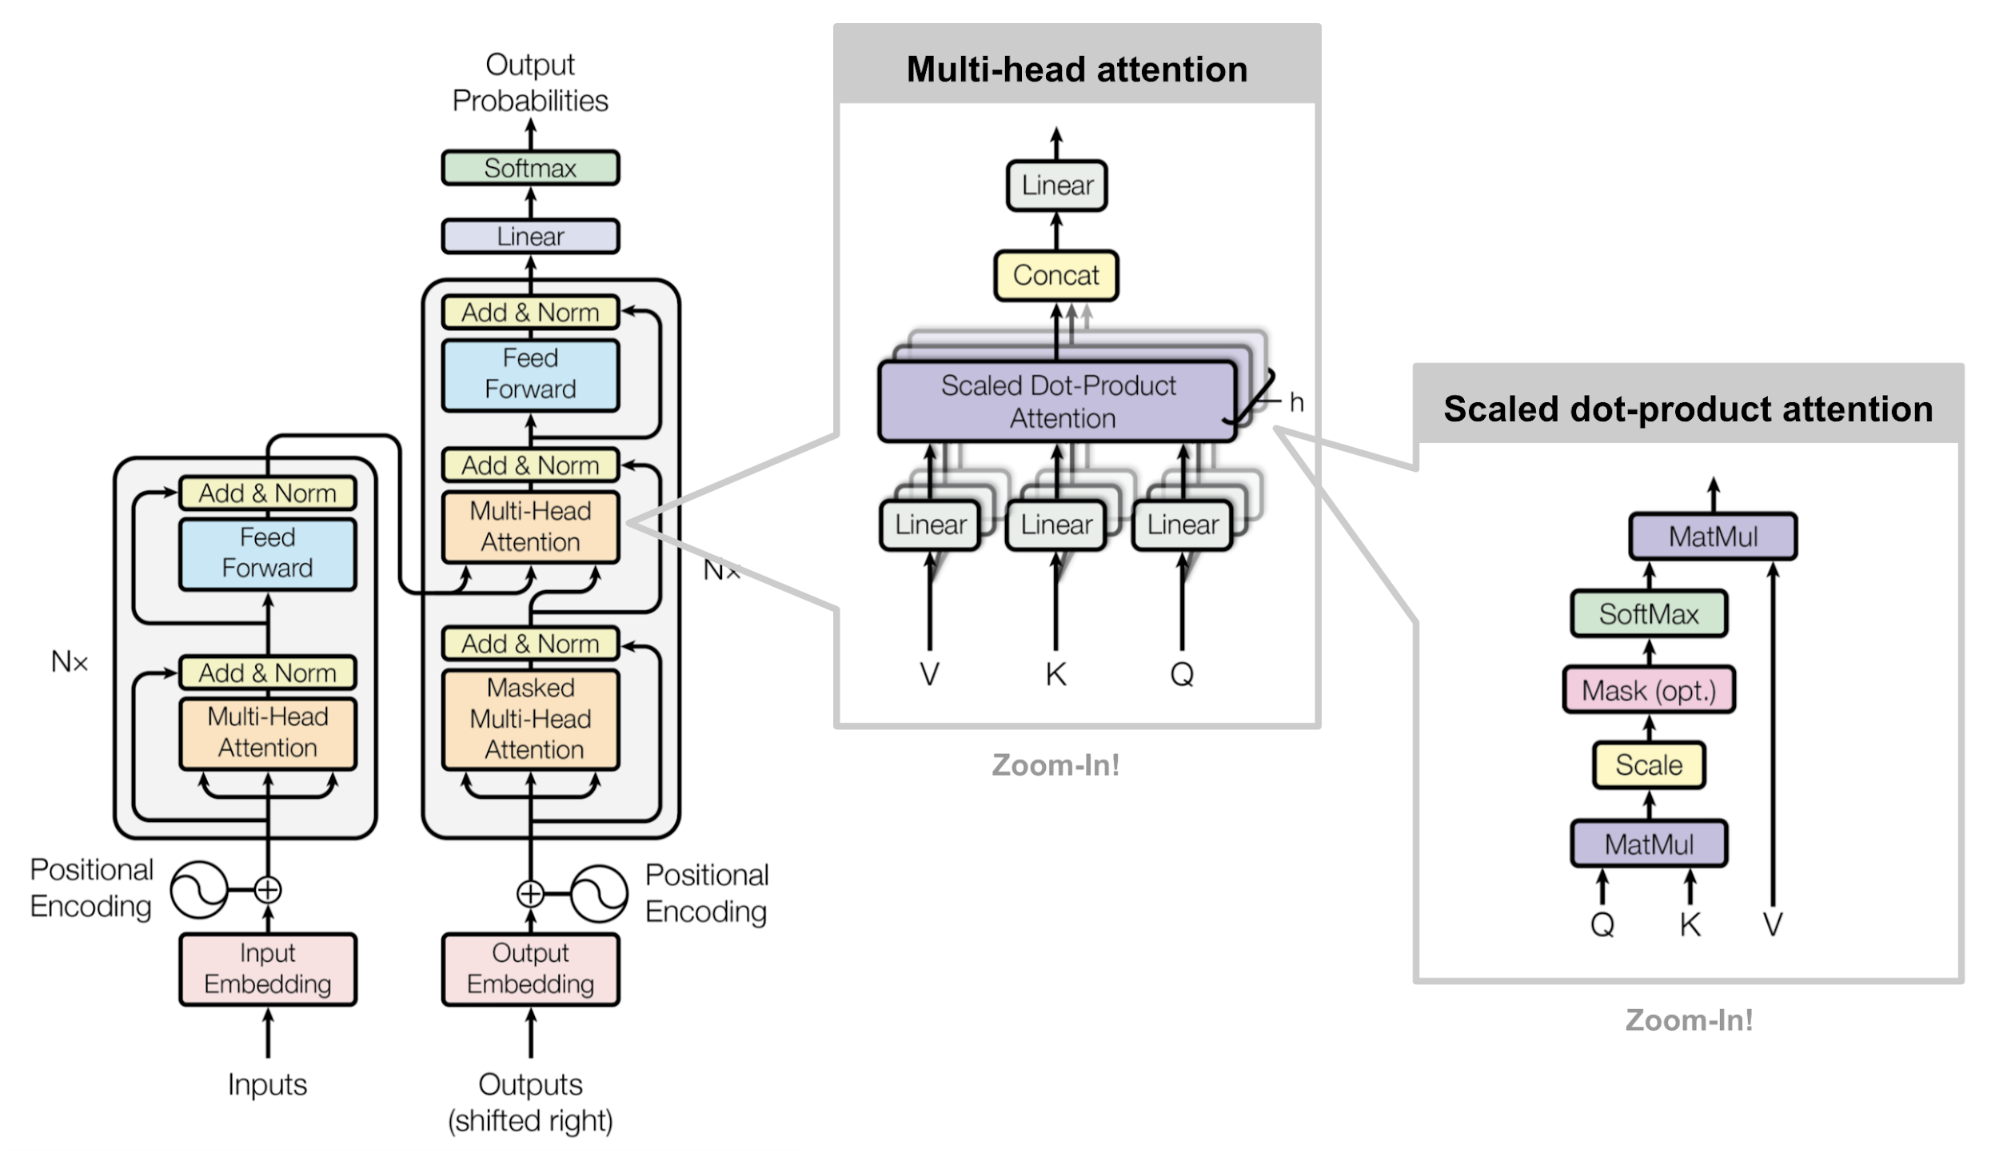
\includegraphics[width=\textwidth]{content/resources/new_images/background/transformer.png}
    \caption{The full transformer architecture \cite{vaswani2017attention}}
    \label{fig:transformer_arch}
\end{figure}


Transformer model has an encoder-decoder architecture. The encoder generates a representation from a large context. It constructed by two main submodules, a \textit{multi-head self-attention} layer and a \textit{projection network}. 

In the transformer decoder is retrieve information from the encoded representation. The architecture is quite similar to the encoder. Figure \ref{fig:transformer_arch} shown the whole propose architecture